\documentclass[tikz]{standalone}
\usepackage[dvipsnames,svgnames,x11names]{xcolor}
\usepackage{tikz}
\usepackage{pgfplots}
\usetikzlibrary{pgfplots.statistics}
\pgfplotsset{compat = 1.12}
\usepackage[
  group-separator={,},
  exponent-product=\cdot,
]{siunitx}
\usepackage{../thesismath}
\begin{document}
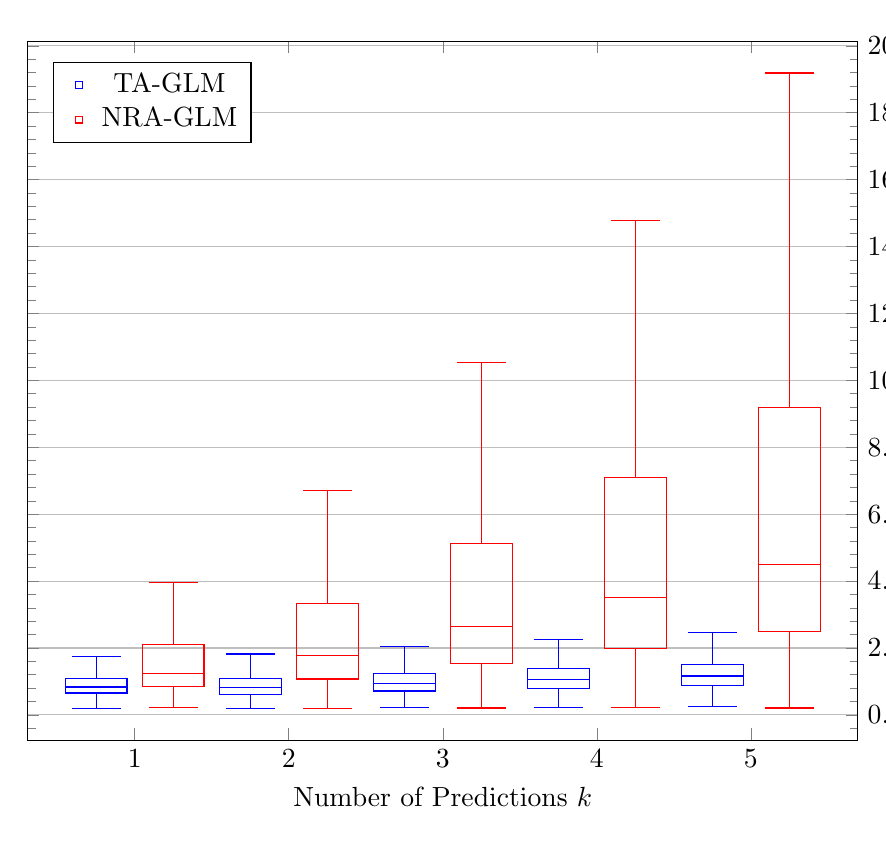
\begin{tikzpicture}[baseline, trim axis left, trim axis right]

\pgfplotscreateplotcyclelist{ta_nra}{%
  blue,  mark size=1.25, mark=square,\\%
  red,   mark size=1.25, mark=square,\\%
}

\pgfplotsset{
  legend style = {
    legend image code/.code = {
      \draw[only marks]
        plot coordinates {
          (0.3cm,0cm)
        };
      \node at (0.15cm, 0cm) {};
      \node at (0.45cm, 0cm) {};
    },
  },
  boxplot/draw/average/.code = {
    % uncomment to show dotted bars for average:
    %\draw[dashed, /pgfplots/boxplot/every average/.try]
    %  (boxplot box cs:\pgfplotsboxplotvalue{average},0)
    %  --
    %  (boxplot box cs:\pgfplotsboxplotvalue{average},1)
    %  ;
  },
}

\sisetup{exponent-base = 2}
\begin{axis}[
%   title = {Calculation Time per top-$1$ Prediction using $5$-grams},
  xlabel = {Number of Predictions $k$},
  xtick = {1, ..., 5},
  ylabel = {Calcluation Time [\si{\milli\second}]},
  yticklabel pos = right,
  ymin = 0.192814,
  ymax = 19.186122,
  scaled x ticks = false,
  scaled y ticks = false,
  minor y tick num = 4,
  y tick label style = {
    /pgf/number format/fixed,
    /pgf/number format/fixed zerofill,
  },
  ymajorgrids = true,
  boxplot/draw direction = y,
  boxplot = {
    box extend = 0.4,
  },
  cycle list name = ta_nra,
  enlargelimits = 0.05,
  legend entries = {{TA-GLM}, {NRA-GLM}},
  legend pos = north west,
  width = \textwidth,
]

% ------------------------------------------------------------------------------

% ngram-5-TA-Weighted-Sum-Generalized-Language-Model-1
\addplot+[
  boxplot prepared = {
    draw position = 0.75,
    lower whisker = 0.202749,
    lower quartile = 0.654436,
    median = 0.832421,
    upper quartile = 1.092418,
    upper whisker = 1.749261,
    average = 0.952469,
  },
] table [row sep = \\, y index = 0] {
  data\\
};

% ngram-5-NRA-Weighted-Sum-Generalized-Language-Model-1
\addplot+[
  boxplot prepared = {
    draw position = 1.25,
    lower whisker = 0.233460,
    lower quartile = 0.843436,
    median = 1.245531,
    upper quartile = 2.091483,
    upper whisker = 3.963493,
    average = 2.339178,
  },
] table [row sep = \\, y index = 0] {
  data\\
};

% ------------------------------------------------------------------------------

% ngram-5-TA-Weighted-Sum-Generalized-Language-Model-2
\addplot+[
  boxplot prepared = {
    draw position = 1.75,
    lower whisker = 0.192814,
    lower quartile = 0.621273,
    median = 0.819823,
    upper quartile = 1.100689,
    upper whisker = 1.819504,
    average = 0.922507,
  },
] table [row sep = \\, y index = 0] {
  data\\
};

% ngram-5-NRA-Weighted-Sum-Generalized-Language-Model-2
\addplot+[
  boxplot prepared = {
    draw position = 2.25,
    lower whisker = 0.192819,
    lower quartile = 1.071781,
    median = 1.786073,
    upper quartile = 3.329700,
    upper whisker = 6.712643,
    average = 4.013765,
  },
] table [row sep = \\, y index = 0] {
  data\\
};


% ------------------------------------------------------------------------------

% ngram-5-TA-Weighted-Sum-Generalized-Language-Model-3
\addplot+[
  boxplot prepared = {
    draw position = 2.75,
    lower whisker = 0.214068,
    lower quartile = 0.714329,
    median = 0.938840,
    upper quartile = 1.250417,
    upper whisker = 2.054324,
    average = 1.040348,
  },
] table [row sep = \\, y index = 0] {
  data\\
};

% ngram-5-NRA-Weighted-Sum-Generalized-Language-Model-3
\addplot+[
  boxplot prepared = {
    draw position = 3.25,
    lower whisker = 0.206416,
    lower quartile = 1.523849,
    median = 2.637291,
    upper quartile = 5.134224,
    upper whisker = 10.545722,
    average = 6.020285,
  },
] table [row sep = \\, y index = 0] {
  data\\
};

% ------------------------------------------------------------------------------

% ngram-5-TA-Weighted-Sum-Generalized-Language-Model-4
\addplot+[
  boxplot prepared = {
    draw position = 3.75,
    lower whisker = 0.222813,
    lower quartile = 0.801222,
    median = 1.049937,
    upper quartile = 1.378405,
    upper whisker = 2.244019,
    average = 1.142494,
  },
] table [row sep = \\, y index = 0] {
  data\\
};

% ngram-5-NRA-Weighted-Sum-Generalized-Language-Model-4
\addplot+[
  boxplot prepared = {
    draw position = 4.25,
    lower whisker = 0.219942,
    lower quartile = 1.995882,
    median = 3.501909,
    upper quartile = 7.108704,
    upper whisker = 14.775368,
    average = 8.298204,
  },
] table [row sep = \\, y index = 0] {
  data\\
};

% ------------------------------------------------------------------------------

% ngram-5-TA-Weighted-Sum-Generalized-Language-Model-5
\addplot+[
  boxplot prepared = {
    draw position = 4.75,
    lower whisker = 0.240061,
    lower quartile = 0.887015,
    median = 1.163096,
    upper quartile = 1.517905,
    upper whisker = 2.464207,
    average = 1.258164,
  },
] table [row sep = \\, y index = 0] {
  data\\
};

% ngram-5-NRA-Weighted-Sum-Generalized-Language-Model-5
\addplot+[
  boxplot prepared = {
    draw position = 5.25,
    lower whisker = 0.206166,
    lower quartile = 2.500258,
    median = 4.498595,
    upper quartile = 9.176688,
    upper whisker = 19.186122,
    average = 11.206972,
  },
] table [row sep = \\, y index = 0] {
  data\\
};

\end{axis}

\end{tikzpicture}
\end{document}
